\documentclass{homework}
\usepackage{cancel}
\author{Michael D. Walker (mw6136), Philip Satterthwaite (ps1639), Michael Schroeder (ms2774)}
\class{APC523: Numerical Algorithms for Scientific Computing}
\date{\today}
\title{Analytical Solution to the Wave Equation in Cylindrical Coordinates}

\begin{document} \maketitle
\subsection{Wave Equation Classification}
The wave equation is a second-order linear partial differential equation (PDE) for the description of waves or standing wave fields. The scalar wave equation describes the mechanical wave propagation of any scalar $\phi$ as 

\[ \frac{\partial^2 \phi}{\partial t^2} = c^2 \left(\frac{\partial^2 \phi}{\partial x^2} + \frac{\partial^2 \phi}{\partial y^2} + \frac{\partial^2 \phi}{\partial z^2}  \right) = c^2 \,\nabla^2 \, \phi \quad ,\]
\noindent
where $c$ is a fixed non-negative real coefficient. $\nabla$ is the \emph{nabla} operator and $\nabla^2 = \nabla \cdot \nabla \equiv \frac{\partial^2}{\partial x^2} + \frac{\partial^2}{\partial y^2} + \frac{\partial^2}{\partial z^2}$ is the spatial Laplacian operator (in Cartesian coordinates). Because the wave equation is linear and homogeneous, it can be analyzed as a linear combination (superposition) of simple solutions that are sinusoidal plane waves with various directions of propagation and wavelengths, but all with the same finite propagation speed $c$. 
\\ \\ \noindent
Projecting the wave equation in the general form of a second-order PDE

\[ A \frac{\partial^2 \phi}{\partial t^2} + B \frac{\partial^2 \phi}{\partial x \partial t} + C \frac{\partial^2 \phi}{\partial x^2} + D \frac{\partial \phi}{\partial t} + E \frac{\partial \phi}{\partial x} + F \phi = 0 \]
\\ \noindent
gives $A = 1$, $B = 0$, and $C = -c^2$, and thus the discriminant $B^2 - 4AC > 0$ defines a hyperbolic PDE with a well-posed initial value problem .

\newpage
\subsection{Algebraic Solution to the 1-D Wave Equation}
The wave equation in one spatial dimension

\[ \frac{\partial^2 \phi}{\partial t^2} = c^2 \, \frac{\partial^2 \phi}{\partial x^2} \]
\\ \noindent
is unusual for a partial differential equation in that a relatively simple general solution may be found. Using an algebraic change of variable $\xi = x - ct$ and  $\eta = x + ct$, and computing the partial derivatives

\begin{align*}
\frac{\partial \phi}{\partial t} &= \frac{\partial \phi}{\partial \xi} \frac{\partial \xi}{\partial t} + \frac{\partial \phi}{\partial \eta} \frac{\partial \eta}{\partial t}
\\
\frac{\partial^2 \phi}{\partial t^2} &= c^2 \frac{\partial^2 \phi}{\partial \xi^2} -2c \frac{\partial^2 \phi}{\partial \xi \partial \eta} + c^2 \frac{\partial^2 \phi}{\partial \eta^2}
\\ \\
\frac{\partial \phi}{\partial x} &= \frac{\partial \phi}{\partial \xi} + \frac{\partial \phi}{\partial \eta}
\\
\frac{\partial^2 \phi}{\partial x^2} &= \frac{\partial^2 \phi}{\partial \xi^2} + 2 \frac{\partial^2 \phi}{\partial \xi \partial \eta} + \frac{\partial^2 \phi}{\partial \eta^2} \quad .
\end{align*}
\noindent
Substituting into the wave equation for $c \neq 0$, the wave equation becomes
\[ \frac{\partial^2 \phi}{\partial \xi \partial \eta }(x,t) = 0 \quad ,\]
which is separable and can be integrated for a general solution, where $F$, $G$, $H$ are arbitrary forcing functions.

\[ \int \frac{\partial^2 \phi}{\partial \xi \partial \eta } \, d \xi = 0 \rightarrow \frac{\partial \phi}{\partial \eta} = H(\eta) \]
\[ \phi(\xi, \eta) = \int \frac{\partial \phi}{\partial \eta} \, d \eta = \int H(\eta) \, d \eta + F(\xi) = F(\xi ) + G(\eta ) \]

\[ \phi(x, t) = F(x - ct) + G(x - ct) \quad .\]
\\ \noindent
Thus the solutions of the 1-D wave equation are sums of a right-translating function $F$ and a left-translating function $G$ at the speed $c$.

\newpage
\subsection{The Wave Equation in Cylindrical Coordinates}
For circularly propagating waves, it is useful to project the wave equation in cylindrical coordinates.

\[ \frac{\partial^2 \phi}{\partial t^2} = c^2 \left(\frac{\partial^2 \phi}{\partial x^2} + \frac{\partial^2 \phi}{\partial y^2} + \frac{\partial^2 \phi}{\partial z^2}  \right) = c^2 \,\nabla^2 \, \phi \]
\\ \noindent
Substituting the transformation from Cartesian variables $(x, y, z)$ to cylindrical $(r, \theta, z)$, $ x = r \cos{\theta}$, $y = r \sin{\theta}$, and $r^2 = x^2 + y^2$, $\theta =\tan^{-1} (y / x)$. 

\begin{figure}[h]
    \begin{center}
    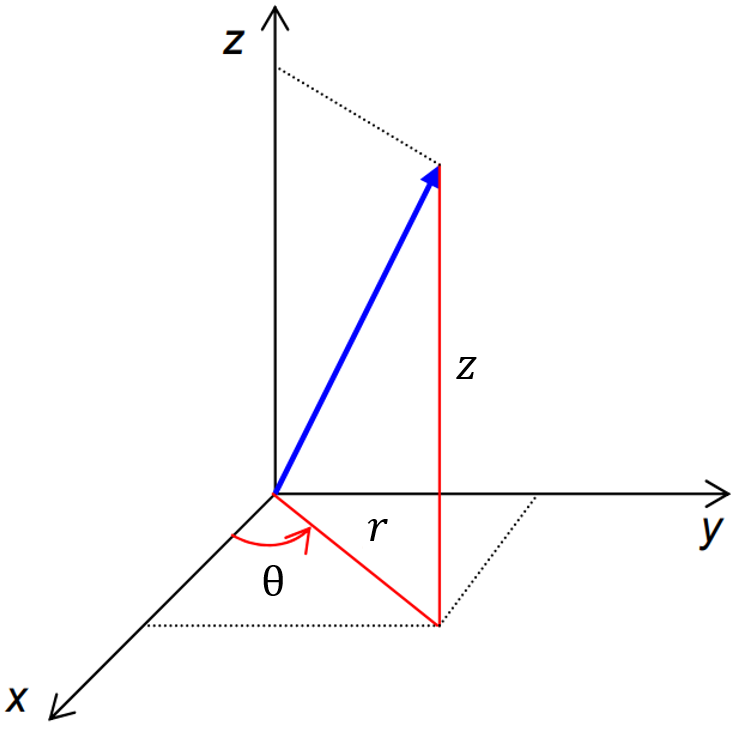
\includegraphics[scale = 0.25]{media/Cylindrical-Coordinates.png}
    \caption{Cartesian and Cylindrical coordinates.}
    \end{center}
\end{figure}
\noindent
The partial derivatives can be evaluated as:
\begin{align*}
\frac{\partial r}{\partial x} &= \frac{x}{r} = \cos(\theta) \qquad \frac{\partial r}{\partial y} = \frac{y}{r} = \sin(\theta) \\
\frac{\partial \theta}{\partial x} &= -\frac{\sin(\theta)}{r} \qquad \quad \; \frac{\partial \theta}{\partial y} = \frac{\cos(\theta)}{r} \\
\end{align*}
\noindent
Applying the chain rule:
\begin{align*}
\frac{\partial \phi}{\partial x} = \frac{\partial \phi}{\partial r} \frac{\partial r}{\partial x} + \frac{\partial \phi}{\partial \theta} \frac{\partial \theta}{\partial x}\\
\frac{\partial \phi}{\partial y} = \frac{\partial \phi}{\partial r} \frac{\partial r}{\partial y} + \frac{\partial \phi}{\partial \theta} \frac{\partial \theta}{\partial y}\\
\end{align*}
\noindent
Therefore, the Laplacian in cylindrical coordinates is

\[ \nabla^2 \;\; = \;\; \frac{\partial^2}{\partial x^2} + \frac{\partial^2}{\partial y^2} + \frac{\partial^2}{\partial z^2} \;\; = \;\; \frac{\partial^2}{\partial r^2} + \frac{1}{r} \frac{\partial}{\partial r} + \frac{1}{r^2} \frac{\partial^2}{\partial \theta^2} + \frac{\partial^2}{\partial z^2} \]
\\ \noindent
and the wave equation can be written as

\[ \frac{1}{c^2} \frac{\partial^2 \phi }{\partial t^2 } = \frac{\partial^2 \phi }{\partial r^2 } + \frac{1}{r} \frac{\partial \phi }{\partial r} + \frac{1}{r^2 } \frac{\partial^2 \phi }{\partial \theta^2 } + \cancel{\frac{\partial^2 \phi }{\partial z^2 }} \quad .\]
\\ \noindent
It is clear that it remains a hyperbolic PDE, but now with a singular point at the origin $r = 0$. The study of surface deformation requires only plane-polar coordinates, so the $\partial^2 \phi / \partial z^2$ term may be neglected. We now seek an analytical solution to the 2-D equation, given well-posed boundary and initial conditions.

\newpage
\subsection{Discretization and Finite Difference Methods}

To discretize the wave equation in polar coordinates, define $r = i \Delta r$, $\theta = j \Delta \theta$, and $t = n \Delta t$. Thus,

$$ \phi \left(r, \theta, t \right)= \phi \left(i \Delta r, j \Delta \theta, n \Delta t \right) = \phi \left(r_i, \theta_j, t^{\left(n\right)} \right) \equiv \phi_{i,j}^{\left(n\right)} $$
where $r_i$ and $\phi_j$ are the positions and $\Delta r$ and $\Delta \theta$ are the cell widths.
\\ \\ \noindent
Considering the Laplacian is divergent at $r=0$:
$$ \nabla^2 = \frac{1}{r} \, \frac{\partial}{\partial r} \left(r \frac{\partial}{\partial r}\right)+ \frac{1}{r^2} \frac{\partial^2}{\partial \theta^2} $$
so too will the discretization diverge. This can be managed in several ways.
\begin{itemize}
    \item Choose a problem such that $r=0$ does not need to be considered (e.g., $r_{\textrm{min}} = 0.001$)
    \item Use cell-centered values for $r$ (e.g., $r_{\textrm{min}} = 0.5 \Delta r$)
    \item Use two meshes: a Cartesian one for $r  \leq 1$ and a polar one for $r \geq 1$, merging them at $r \simeq 1 $ (requires at least 1 cell of overlap).
\end{itemize}

\subsubsection{Explicit (forward difference) methods}

Using the forward difference in $r$ and central differences in $\theta$ and $t$,
\begin{align*}
    \frac{1}{r} \, \frac{\partial}{\partial r}\left(r \frac{\partial \phi}{\partial r} \right) &= \frac{1}{r_i} \left(r_{i+1/2} \frac{\phi^{\left(n\right)}_{i+1,j} - \phi^{\left(n\right)}_{i,j}}{\Delta r^2} - r_{i-1/2} \frac{\phi^{\left(n\right)}_{i,j} - \phi^{\left(n\right)}_{i-1,j}}{\Delta r^2} \right) \\
    \frac{1}{r^2} \frac{\partial^2\phi}{\partial \theta^2} &= \frac{1}{{r_i}^2} \left( \frac{\phi^{\left(n\right)}_{i,j+1} - 2 \phi^{\left(n\right)}_{i,j} + \phi^{\left(n\right)}_{i,j-1}}{{\Delta \theta}^2} \right)
\end{align*}
\\ \noindent
where $r_{i + 1/2}= 0.5 \left(r_{i+1} + r_i \right)$. Thus the full wave equation
\begin{align*}
    \phi_{i,j}^{\left(n+1\right)} &= 2 \phi_{i,j}^{\left(n\right)} - \phi_{i,j}^{\left(n-1\right)} \\
    &+ \frac{c^2 \Delta t^2}{\Delta r^2}\left[\phi_{i+2,j}^{\left(n\right)} + \frac{1}{i}\phi_{i+2,j}^{\left(n\right)} - 2\phi_{i+1,j}^{\left(n\right)} - \frac{1}{i}\phi_{i+1,j}^{\left(n\right)} + \phi_{i,j}^{\left(n\right)}\right] \\
    &+ \frac{c^2 \Delta t^2}{i^2 \Delta r^2 {\Delta \theta}^2} \left[\phi_{i,j+1}^{\left(n\right)} + \phi_{i,j-1}^{\left(n\right)} - 2\phi_{i,j}^{\left(n\right)} \right]
\end{align*}
\\ \noindent
The spatial discretization is $\Delta r$, $\Delta \theta$ is user defined. The timestep $\Delta t$ is limited by the Courant-Friedrichs-Levy (CFL) condition. For the wave equation, such that
$$ c^2 \frac{\Delta t}{\min(\Delta r^2, {\Delta \theta}^2)} \leq \frac{1}{2} $$
Where formally the constant is limited by the dimensionality of the system $ 1 / N_{\textrm{dim}}$. For time-stepping purposes, this is the speed limitation of the algorithm. Thus, for performance, it is worthwhile to consider Implicit methods.

\subsubsection{Implicit (backward difference) methods}
\subsubsection{Crank–Nicolson scheme}
To summarize, usually the Crank–Nicolson scheme is the most accurate scheme for small time steps. For larger time steps, the implicit scheme works better since it is less computationally demanding. The explicit scheme is the least accurate and can be unstable, but is also the easiest to implement and the least numerically intensive.

\newpage
\subsection{\textbf{Problem Statement}}
\noindent Note: this problem was adapted from Problem Set 9, Exercise 3 of Princeton University Course MAE501: Mathematical Methods of Engineering Analysis I given in Fall semester 2023.
\\ \\
\noindent For a small deformation of any planar circular elastic material, the surface deformation, $\phi$, satisfies the wave equation in plane-polar coordinates

\[ \frac{\partial^2 \phi}{\partial t^2} = c^2 \left[ \frac{1}{r} \frac{\partial}{\partial r} \left(r \frac{\partial \phi}{\partial r}\right) + \frac{1}{r^2} \frac{\partial^2 \phi}{\partial \theta^2} \right]\]
\\
\noindent where the driving force of the wave motion for a material initially at rest can be specified through the boundary and initial conditions. Seeking to model waves on the surface of the fluid generated by the motion of the walls, we choose the following boundary and initial conditions. \\ \\
\noindent Boundary Conditions: \\
$ \phi(r=R, \theta, t) = A \cos(\omega t) \cos (\theta) $ \\
$ \phi(r=0, \theta, t) \rightarrow \textrm{finite} $ \\
$ \phi(r, \theta + 2\pi, t) = \phi(r, \theta, t) $ \\ \\
\noindent Initial Conditions: \\
$ \phi(r, \theta, t=0) = 0 $ \\
$ \partial \phi/ \partial t \, (r, \theta, t=0) = 0 $

\subsection{Method of Solution}
We will solve for $\phi$ for all $t$, $\theta$, and $r$ using the method of separation of variables and eigenfunction expansions. We will also determine the resonance condition for the value of $\omega$. 
\\ \\
\noindent Steps in the solution:
\begin{enumerate}
    \item Use Separation of Variables to de-couple the time component and determine the eigenfunctions for the operator with boundary conditions
    \[ \nabla^2 \psi = \left[ \frac{1}{r} \frac{\partial}{\partial r} \left(r \frac{\partial \psi}{\partial r}\right) + \frac{1}{r^2} \frac{\partial^2 \psi}{\partial \theta^2} \right] = - \lambda \psi \]
    \noindent Boundary Conditions: \\
    $ \psi(r=R, \theta) = 0 $ \\
    $ \psi(r=0, \theta) \rightarrow \textrm{finite} $ \\
    $ \psi(r, \theta + 2\pi) = \psi(r, \theta) $ \\
    \item Determine a function $\tilde{\phi}$, that when subtracted from $\phi$ makes the boundary conditions homogeneous but perhaps introduces inhomogeneities in the initial conditions and the equation itself.
    \item Use the eigenfunctions determined from the separation of variables in the method of eigenfunction expansions and solve for $\phi$.
\end{enumerate} 

\newpage
\subsection{Final Solution}
\noindent These conditions lead to the analytical solution 
$$ \phi(r, \theta, t) = A \left(\frac{r}{R} \right)^2 \cos(\omega t) \cos(\theta) + \tilde{\phi} (r, \theta, t)$$ 

\noindent $\tilde{\phi}$ is composed as follows, where $J_\alpha (\cdot)$ is the Bessel function of the 1st kind and order $\alpha$, $\eta$ is a variable of integration, and $\lambda$ are the eigenfunctions for each of the modes.
$$ \tilde{\phi} (r, \theta, t) = \sum_{m=1}^\infty \Biggl( \frac{1}{c^2 \lambda_{n,m} - \omega^2} \frac{2A}{R^2} \frac{\int_0^1 \left( \omega^2 \eta^2 + 3c^2 \right) \eta J_1\left( \sqrt{\lambda_{1,m}} R \eta \right) d\eta }{{J_2}^2 \left( \sqrt{\lambda_{1,m}} R \right)} \cos(\omega t) \; \dots $$

$$ - \frac{2A}{{J_2}^2 \left( \sqrt{\lambda_{1,m}} R \right)}\Bigg[ \int_0^1 \eta^3 J_1 \left( \sqrt{\lambda_{1,m}} R\eta \right) d\eta \; \dots $$

$$ + \frac{1}{c^2 \lambda_{n,m} - \omega^2} \frac{1}{R^2} \int_0^1 \left(\omega^2 \eta^2 + 3c^2 \right) \eta J_1 \left(\sqrt{\lambda_{1,m}} R \eta \right) d\eta \Bigg] \cos \left(c \sqrt{\lambda_{1,m}} t \right) \Biggl) \cos(\theta) J_1 \left(\sqrt{\lambda_{1,m} } r \right) .$$

\subsection{Full Derivation}
\noindent The method of Separation of Variables can be applied to a partial differential equation (PDE) when the equation is linear and homogeneous, where the boundary conditions are also linear and homogeneous. Thus, considering the homogeneous stationary boundary value problem, using separation of variables, assume $\phi(r, \theta, t) = \psi (r, \theta) \mathcal{T} (t)$ and substituting in the wave equation

\[ \frac{\partial^2 (\psi \mathcal{T})}{\partial t^2} = c^2 \left[ \frac{1}{r} \frac{\partial}{\partial r} \left(r \frac{\partial (\psi \mathcal{T})}{\partial r}\right) + \frac{1}{r^2} \frac{\partial^2 (\psi \mathcal{T})}{\partial \theta^2} \right] \quad \rightarrow \quad \psi \mathcal{T}'' = c^2 \left[ \frac{\mathcal{T}}{r} \frac{\partial}{\partial r} \left(r \frac{\partial \psi}{\partial r}\right) + \frac{\mathcal{T}}{r^2} \frac{\partial^2 \psi}{\partial \theta^2} \right] \quad .\]
\\ \noindent
Dividing by $\psi \mathcal{T} c^2$,

\[ \frac{1}{\psi} \left[ \frac{1}{r} \frac{\partial}{\partial r} \left(r \frac{\partial \psi}{\partial r}\right) + \frac{1}{r^2} \frac{\partial^2 \psi}{\partial \theta^2} \right] = \frac{1}{c^2} \frac{\mathcal{T}''}{\mathcal{T}} = - \lambda \quad ,\]
\\ \noindent
with $\lambda$ a constant that will be shown to correspond to the eigenfunctions for each of the modes. Now using separation of variables again on the spatial component, assume $ \psi (r, \theta) = \mathcal{R}(r) \, \Theta(\theta) $ and again substitute into the $\nabla^2 \psi$ operator

\[ \frac{1}{r} \frac{\partial}{\partial r} \left(r \frac{\partial (\mathcal{R} \Theta)}{\partial r}\right) + \frac{1}{r^2} \frac{\partial^2 (\mathcal{R} \Theta)}{\partial \theta^2} = - \lambda \mathcal{R} \Theta \quad \rightarrow \quad \frac{\Theta}{r} (\mathcal{R}' + r \mathcal{R}'') + \frac{\mathcal{R} \Theta''}{r^2} = - \lambda \mathcal{R} \Theta \quad .\]
\noindent
The PDE can then be rewritten as

\[ \frac{1}{\mathcal{R}} r \frac{d}{dr} \big(r \mathcal{R'} \big) + \lambda r^2 = -\frac{\Theta''}{\Theta}  = \alpha^2 \]
\\ \noindent
with $\alpha^2$ as some constant. First solving the angular component by applying an integrating factor and solving for the roots of the characteristic polynomial $\Theta \sim \exp(\delta \theta) \rightarrow \delta = \pm \alpha i$, then substituting Euler's identity $\exp(i \alpha) = \cos(\alpha) + i \, \sin(\alpha)$. 

\[ \Theta'' = -\alpha^2 \Theta \quad \rightarrow \quad \Theta (\theta) = a \cos(\alpha \theta) + b \sin(\alpha \theta) \quad .\]
\noindent
Applying the condition $\psi(r, \theta + 2\pi) = \psi(r, \theta)$,
\begin{equation*}
    \begin{split}
        a &\cos(\alpha \theta + \alpha 2 \pi) + b \sin(\alpha \theta + \alpha 2 \pi) = a \cos(\alpha \theta) + b \sin(\alpha \theta) \\
        &\rightarrow  \cos(\alpha \theta + \alpha 2 \pi) = \cos(\alpha \theta) \quad \textrm{and} \quad \sin(\alpha \theta + \alpha 2 \pi) = \sin(\alpha \theta) \\
        &\rightarrow \alpha_n = n \in \mathbb{Z}^{\geq 0} \;\; \textrm{an integer}
    \end{split}
\end{equation*}

\noindent
Therefore a solution to the angular problem is

\[\Theta_n (\theta) = a_n \cos(n \theta) + b_n \sin(n \theta) \quad . \]
\newpage
\noindent
Now re-arranging the radial problem (where the substitution $\alpha_n = n$) is made,

\[ \frac{1}{\mathcal{R}} r \frac{d}{dr} \big(r \mathcal{R'} \big) + \lambda r^2 = n^2 \quad \rightarrow \quad r \frac{d}{dr} \big(r \mathcal{R'} \big) + (\lambda r^2 - n^2) \mathcal{R} = 0 \]

\[ r^2 \mathcal{R}'' + r \mathcal{R}' + (\lambda r^2 - n^2) \mathcal{R} = 0 \]
\noindent 
This is the form of a Bessel equation of order $n$ and therefore the solutions to the radial problem are the Bessel functions of order $n$,

\[\mathcal{R}(r) = c J_n (\sqrt{\lambda} r) + d \cancel{Y_n (\sqrt{\lambda} r)} \quad .\]

\noindent
Applying boundary conditions: \\
\noindent $\mathcal{R}(r = 0) \; \textrm{finite} \; \rightarrow \; d = 0$ \\
\noindent $\mathcal{R}(r = R) = 0 \; \rightarrow \; c J_n (\sqrt{\lambda_{n,m}} r) = 0 \; \rightarrow \; \sqrt{\lambda_{n,m}} r = z_{n,m} \; \textrm{for} \; c \neq 0$ \\ \\ \noindent
This gives a relation between the eigenvalues and zeroes of the Bessel function,  where $z_{n,m}$ is the $m$-th zero of the $n$-th order Bessel function $J_n$ for $m = 1,2,3 \dots$ Therefore the eigenfunctions  are of the form 

\[ \psi_{n,m} (r, \theta) = \mathcal{R}(r) \, \Theta(\theta) = [a_{n,m} \cos(n \theta) + b_{n,m} \sin(n \theta)] J_n (\sqrt{\lambda_{n,m}} r) \]
\\ \noindent
With the modes of $a_{n,m}(t)$ and $b_{n,m}(t)$ to be determined as functions of time. Now considering the original problem, the boundary condition is inhomogeneous, so we must rescale the problem to achieve homogeneous boundary conditions. Let

\[ \tilde{\phi} \equiv \phi - A \left(\frac{r}{R} \right)^2 \cos(\omega t) \cos(\theta) \]
\noindent
Here the $r^2 / R^2$ term is necessary to resolve the singularity from the ODE. Taking the time and spatial derivatives of $\tilde{\phi}$ to rewrite the PDE:

\begin{align*}
\frac{ \partial \phi}{\partial t} &= \frac{ \partial \tilde{\phi}}{\partial t} - A \omega \left(\frac{r}{R} \right)^2 \sin(\omega t) \cos(\theta) \\
\frac{ \partial \phi}{\partial r} &= \frac{ \partial \tilde{\phi}}{\partial r} - 2 A \left(\frac{r}{R^2}\right) \cos(\omega t) \cos(\theta) \\
\frac{ \partial^2 \phi}{\partial t^2} &= \frac{ \partial^2 \tilde{\phi}}{\partial t^2} - A \omega^2 \left(\frac{r}{R} \right)^2 \cos(\omega t) \cos(\theta) \\
\frac{1}{r} \frac{\partial}{\partial r} (r \frac{\partial \phi}{\partial r}) &= \frac{1}{r} \frac{\partial}{\partial r} (r \frac{\partial \tilde{\phi}}{\partial r}) + 4 A \left(\frac{1}{R^2}\right) \cos(\omega t) \cos(\theta) \\
\frac{1}{r^2} \frac{\partial^2 \phi }{\partial \theta^2} &= \frac{1}{r^2} \frac{\partial^2 \tilde{\phi} }{\partial \theta^2} - A \left(\frac{1}{R^2}\right) \cos(\omega t) \cos(\theta)
\end{align*}
\noindent
Now combining to rewrite the solution in terms of the transformed variable $\tilde{\phi}$,

\[ \frac{ \partial^2 \tilde{\phi}}{\partial t^2} - A \omega^2 \left(\frac{r}{R} \right)^2 \cos(\omega t) \cos(\theta) = c^2 \left[ \frac{1}{r} \frac{\partial}{\partial r} (r \frac{\partial \tilde{\phi}}{\partial r}) + \frac{4A}{R^2} \cos(\omega t) \cos(\theta) + \frac{1}{r^2} \frac{\partial^2 \tilde{\phi} }{\partial \theta^2} - \frac{A}{R^2} \cos(\omega t) \cos(\theta) \right]\]
\noindent
which simplifies as

\[ \frac{ \partial^2 \tilde{\phi}}{\partial t^2} - \frac{A}{R^2} \cos(\omega t) \cos(\theta) (\omega^2 r^2 + 3c^2) = c^2 \left[ \frac{1}{r} \frac{\partial}{\partial r} (r \frac{\partial \tilde{\phi}}{\partial r}) + \frac{1}{r^2} \frac{\partial^2 \tilde{\phi} }{\partial \theta^2} \right] \quad .\]
\newpage
\noindent
The initial and boundary conditions are similarly re-scaled.
\\ \\
\noindent Boundary Conditions: \\
$ \tilde{\phi}(r=R, \theta, t) = 0 $ \\
$ \tilde{\phi}(r=0, \theta, t) \rightarrow \textrm{finite} $ \\
$ \tilde{\phi}(r, \theta + 2\pi, t) = \tilde{\phi}(r, \theta, t) $ \\ \\
\noindent Initial Conditions: \\
$ \tilde{\phi}(r, \theta, t=0) = - A \left( \frac{r^2}{R^2} \right) \cos(\theta) $ \\
$ \partial \tilde{\phi}/ \partial t \, (r, \theta, t=0) = 0 $ \\ \\ \noindent
Note that the boundary conditions are now homogeneous, but one of the initial conditions is inhomogeneous. For convenience, define a function

\[ f(r, \theta , t) \equiv A \left( \frac{1}{R^2} \cos(\omega t) \cos(\theta) (\omega^2 r^2 + 3c^2) \right) \quad .\]
\noindent
Solving the new PDE in $\tilde{\phi}$ we expand the inhomogeneity $f(r, \theta , t)$ in the eigenfunctions of the stationary problem

\[ f(r, \theta , t) = \sum^\infty_{n=0} \sum^\infty_{m=0} [c_{n,m}(t) \cos(n \theta) + d_{n,m}(t) \sin(n \theta) ] J_n (\sqrt{\lambda_{n,m}} r) \]
\noindent
Using orthogonality of eigenfunctions we can solve for $c_{n,m}(t)$ and $d_{n,m}(t)$ by calculating the inner product using an appropriate weight function $r$

\[ c_{n,m}(t) = \frac{\langle f(r, \theta, t), J_n (\sqrt{\lambda_{n,m}} r) \cos(n \theta) \rangle_r}{\langle J_n (\sqrt{\lambda_{n,m}} r) \cos(n \theta), J_n (\sqrt{\lambda_{n,m}} r) \cos(n \theta) \rangle_r} = \frac{\int^R_0 \int^{2 \pi}_0 f(r, \theta , t) r J_n (\sqrt{\lambda_{n,m}} r) \cos(n \theta) dr \, d \theta}{\int^R_0 \int^{2 \pi}_0 r {J_n}^2 (\sqrt{\lambda_{n,m}} r) \cos^2(n \theta) dr \, d \theta} \]
\[ d_{n,m}(t) = \frac{\langle f(r, \theta, t), J_n (\sqrt{\lambda_{n,m}} r) \sin(n \theta) \rangle_r}{\langle J_n (\sqrt{\lambda_{n,m}} r) \sin(n \theta), J_n (\sqrt{\lambda_{n,m}} r) \sin(n \theta) \rangle_r} = \frac{\int^R_0 \int^{2 \pi}_0 f(r, \theta , t) r J_n (\sqrt{\lambda_{n,m}} r) \sin(n \theta) dr \, d \theta}{\int^R_0 \int^{2 \pi}_0 r {J_n}^2 (\sqrt{\lambda_{n,m}} r) \sin^2(n \theta) dr \, d \theta} \]
\noindent
We can rewrite 

\begin{multline*}
\int^R_0 \int^{2 \pi}_0 f(r, \theta , t) \, r J_n (\sqrt{\lambda_{n,m}} r) \cos(n \theta) \, dr \, d \theta \;=\\ \frac{A}{R^2} \cos(\omega t) \left[ \int^{2 \pi}_0 \cos(\theta) \cos(n \theta) \, d \theta \int^R_0 (\omega^2 r^2 + 3c^2)  r J_n (\sqrt{\lambda_{n,m}} r) \, d r \right]
\end{multline*}
\noindent
Because $\cos(n \theta)$ are orthogonal functions, only when $n = 1$ is $c_{n,m}$ non-zero.

\[ \int^{2 \pi}_0 \cos(\theta) \cos(n \theta) d \theta = 
\begin{cases}
      \pi & \text{if $n=1$}\\
      0 & \text{if $n \neq 1$}\\
    \end{cases}
\]
\noindent
Thus $c_{n,m}$ simplifies to 

\[ c_{n,m} = 
\begin{cases}
      0 & \text{if $n \neq 1$}\\
      \frac{2A}{R^4} \cos(\omega t) \frac{\int^R_0 (\omega^2 r^2 + 3c^2)  r J_1 (\sqrt{\lambda_{1,m}} r) \, d r}{{J_2}^2 (\sqrt{\lambda_{1,m}} R) } & \text{if $n = 1$}\\
    \end{cases}
\]
\noindent
This also requires the integration property of Bessel functions $\int x^n J_{n-1}(x) dx = x^n J_n(x)$. Similarly, as $f(r, \theta, t)$ is only a function of cosine, 

\[ \int^{2 \pi}_0 \cos(\theta) \sin(n \theta) d \theta = 0 \,\forall \, n \quad \rightarrow \quad d_{n,m} = 0 \; .\]
\newpage
\noindent
Since $\cos(\theta)$ corresponds to $m = 1$ and $\cos(n \theta)$ is orthogonal to $\cos(m \theta)$ for $ n \neq m$, all terms $n \neq 1$ are 0 and the summation over $n$ can be removed.

\[ f(r, \theta , t) = \frac{2A}{R^4} \cos(\omega t) \sum^\infty_{m=1} \frac{\int^R_0 (\omega^2 \zeta^2 + 3c^2)  \zeta J_1 (\sqrt{\lambda_{1,m}} \zeta) d \zeta}{{J_2}^2 (\sqrt{\lambda_{1,m}} R) } \cos(\theta) J_1(\sqrt{\lambda_{n,m}} r)\]
\noindent
Here $\zeta$ is the variable of integration. If we non-dimensionalize the variable in the integral with $R \eta = \zeta$,

\[ f(r, \theta , t) = \frac{2A}{R^2} \cos(\omega t) \sum^\infty_{m=1} \frac{\int^1_0 (\omega^2 \eta^2 + 3c^2)  \eta J_1 (\sqrt{\lambda_{1,m}} R \eta) d \eta}{{J_2}^2 (\sqrt{\lambda_{1,m}} R) } \cos(\theta) J_1(\sqrt{\lambda_{n,m}} r) \quad .\]
\\ \noindent
Similar to the stationary problem, the eigenfunction expansion of $\tilde{\phi}(r, \theta , t)$ is

\[ \tilde{\phi}(r, \theta , t) = \sum^\infty_{n=0} \sum^\infty_{m=1} [a_{n,m}(t) \cos(n \theta) + b_{n,m}(t) \sin(n \theta) ] J_n (\sqrt{\lambda_{n,m}} r) \quad . \]
\\ \noindent
Then we can deduce the following ODE relationships from the PDE:
\begin{align*}
n \neq 1 &: a_{n,m}''(t) = -\lambda_{n,m} \, c^2 \, a_{n,m}(t) \\
n = 1 &: a_{1,m}''(t) - c_{1,m}(t) = -\lambda_{1,m} \, c^2 \, a_{1,m}(t) \\
\forall \, n &: b_{n,m}''(t) = -\lambda_{n,m} \, c^2 \, b_{n,m}(t) \\
\end{align*}
\noindent
Now using the initial conditions for the PDE to get initial conditions for these coefficient ODEs

\[ \tilde{\phi}(r, \theta , t=0) = -A \, \frac{r^2}{R^2} \cos(\theta) \sum^\infty_{n=0} \sum^\infty_{m=1} [a_{n,m}(0) \cos(n \theta) + b_{n,m}(0) \sin(n \theta) ] J_n (\sqrt{\lambda_{n,m}} r) \quad .\]
\noindent
The initial condition does not have a $\sin(\theta)$ term and therefore $b_{n,m}(0) = 0$. To solve for $a_{n,m}(0)$, we use orthogonality of eigenfunctions and take inner products of both sides with $\cos(n \theta) J_n(\sqrt{\lambda_{n,m}} r)$ and using an appropriate weight function $r$

\begin{align*}
a_{n,m}(0) &= \frac{\langle -A \, \frac{r^2}{R^2} \cos(\theta), J_n(\sqrt{\lambda_{n,m}} r) \cos(n \theta) \rangle_r}{\langle J_n(\sqrt{\lambda_{n,m}} r) \cos(n \theta), J_n(\sqrt{\lambda_{n,m}} r) \cos(n \theta) \rangle_r} \\
&= \frac{\int^R_0 \int^{2 \pi}_0 -A (\frac{r}{R})^2 \cos(\theta) r J_n (\sqrt{\lambda_{n,m}} r) \cos(n \theta) \, dr \, d \theta}{\int^R_0 \int^{2 \pi}_0 r {J_n}^2 (\sqrt{\lambda_{n,m}} r) \cos^2(n \theta) \, dr \, d \theta} \\
&= \frac{\int^R_0 -A (\frac{r}{R})^2 r J_n (\sqrt{\lambda_{n,m}} r) \, dr \int^{2 \pi}_0 \cos(\theta) \cos(n \theta) \, d \theta}{\frac{1}{2} \pi R^2 {J_2}^2 (\sqrt{\lambda_{n,m}} R)}
\end{align*}

\begin{align*}
    &= \begin{cases}
    0 & \textrm{if $n \neq 1$} \\
    \frac{-2A}{R^4 J_{n+1}^2 (\sqrt{\lambda_{n,m}} R)} \int^R_0 r^3 J_1 (\sqrt{\lambda_{1,m}} r) \, dr & \textrm{if $n = 1$}
    \end{cases} \\
    &= \begin{cases}
    0 & \textrm{if $n \neq 1$} \\
    \frac{-2A}{{J_2}^2 (\sqrt{\lambda_{n,m}} R)} \int^1_0 \eta^3 J_1 (\sqrt{\lambda_{1,m}} R \eta) \, d \eta & \textrm{if $n = 1$}
    \end{cases}
\end{align*}
\noindent
This also requires the integration property of Bessel functions $\int x^n J_{n-1}(x) dx = x^n J_n(x)$. Applying the second initial condition

\[ \frac{\partial \tilde{\phi}}{\partial t}(r, \theta , t=0) = 0 = \sum^\infty_{n=0} \sum^\infty_{m=1} [a_{n,m}'(0) \cos(n \theta) + b_{n,m}'(0) \sin(n \theta) ] J_n (\sqrt{\lambda_{n,m}} r) \]
\\ \noindent
implies that $a_{n,m}'(0) = 0$ and $b_{n,m}'(0) = 0$. Now solving the ODEs for $a_{n,m}$ and $b_{n,m}$. First for the case $n \neq 1$, by applying an integrating factor and solving for the roots of the characteristic polynomial $a \sim \exp(\delta t) \rightarrow \delta = \pm c \sqrt{\lambda_{n,m}} i$, then substituting Euler's identity $\exp(i c \sqrt{\lambda_{n,m}} t) = \cos(c \sqrt{\lambda_{n,m}} t) + i \, \sin(c \sqrt{\lambda_{n,m}} t)$. We use the initial conditions to solve for the constants $\kappa_1$, $\kappa_2$

\[ a_{n,m}(t) = \kappa_1 \cos(c \sqrt{\lambda_{n,m}} t) + \kappa_2 \sin(c \sqrt{\lambda_{n,m}} t) \quad \rightarrow \quad \kappa_1 = 0, \; \kappa_2 = 0 \quad \rightarrow \quad a_{n,m}(t) = 0\]
\\ \noindent
Similarly for all $n$, $b_{n,m}(t) = 0$. For the case $n = 1$:

\[ a_{n,m}''(t) = \frac{2A}{R^2} \cos(\omega t) \, \frac{\int_0^1 \left( \omega^2 \eta^2 + 3c^2 \right) \eta J_1\left( \sqrt{\lambda_{1,m}} R \eta \right) d\eta}{{J_2}^2 \left( \sqrt{\lambda_{1,m}} R \right)} = -c^2 \lambda_{n,m} a_{1,m} \]
\noindent
The homogeneous solution to this ODE is of the form (again using an integrating factor approach)

\[ a_{n,m}^{\textrm{hom}}(t) = \kappa_3 \cos(c \sqrt{\lambda_{n,m}} t) + \kappa_4 \sin(c \sqrt{\lambda_{n,m}} t) \]
\noindent
and by inspection we find a particular solution

\[ a_{n,m}^{\textrm{part}}(t) = \kappa_5 \cos(\omega t) \quad .\]
\noindent
Solving for $k_5$ yields

\[ \kappa_5 = \frac{1}{c^2 \lambda_{n,m} - \omega^2} \frac{2A}{R^2} \frac{\int_0^1 \left( \omega^2 \eta^2 + 3c^2 \right) \eta J_1\left( \sqrt{\lambda_{1,m}} R \eta \right) d\eta}{{J_2}^2 \left( \sqrt{\lambda_{1,m}} R \right)} \quad .\]
\noindent
The general solution for the coefficients is thus

\[ a_{1,m}(t) = \kappa_3 \cos(c \sqrt{\lambda_{n,m}} t) + \kappa_4 \sin(c \sqrt{\lambda_{n,m}} t) + \frac{1}{c^2 \lambda_{n,m} - \omega^2} \frac{2A}{R^2} \frac{\int_0^1 \left( \omega^2 \eta^2 + 3c^2 \right) \eta J_1\left( \sqrt{\lambda_{1,m}} R \eta \right) d\eta}{{J_2}^2 \left( \sqrt{\lambda_{1,m}} R \right)} \cos(\omega t) \; .\]
\noindent
From the initial conditions we find that $\kappa_4 = 0$ and

\[ \kappa_3 = \frac{-2A}{{J_2}^2 \left( \sqrt{\lambda_{1,m}} R \right)} \int_0^1 \eta^3 J_1 \left( \sqrt{\lambda_{1,m}} R \eta \right) d \eta - \frac{1}{c^2 \lambda_{n,m} - \omega^2} \frac{2A}{R^2} \frac{\int_0^1 \left( \omega^2 \eta^2 + 3c^2 \right) \eta J_1\left( \sqrt{\lambda_{1,m}} R \eta \right) d\eta }{{J_2}^2 \left( \sqrt{\lambda_{1,m}} R \right)}\]
\noindent
\textbf{Substituting to write the closed form solution for $\tilde{\phi}$}

$$ \tilde{\phi} (r, \theta, t) = \sum_{m=1}^\infty \Biggl( \frac{1}{c^2 \lambda_{n,m} - \omega^2} \frac{2A}{R^2} \frac{\int_0^1 \left( \omega^2 \eta^2 + 3c^2 \right) \eta J_1\left( \sqrt{\lambda_{1,m}} R \eta \right) d\eta }{{J_2}^2 \left( \sqrt{\lambda_{1,m}} R \right)} \cos(\omega t) \; \dots $$

$$ - \frac{2A}{{J_2}^2 \left( \sqrt{\lambda_{1,m}} R \right)}\Bigg[ \int_0^1 \eta^3 J_1 \left( \sqrt{\lambda_{1,m}} R\eta \right) d\eta \; \dots $$

$$ + \frac{1}{c^2 \lambda_{n,m} - \omega^2} \frac{1}{R^2} \int_0^1 \left(\omega^2 \eta^2 + 3c^2 \right) \eta J_1 \left(\sqrt{\lambda_{1,m}} R \eta \right) d\eta \Bigg] \cos \left(c \sqrt{\lambda_{1,m}} t \right) \Biggl) \cos(\theta) J_1 \left(\sqrt{\lambda_{1,m} } r \right) .$$
\noindent
\textbf{and the solution in the original variable}
$$ \phi(r, \theta, t) = A \left(\frac{r}{R} \right)^2 \cos(\omega t) \cos(\theta) + \tilde{\phi} (r, \theta, t) \quad .$$ 

\noindent By inspection of $\tilde{\phi}(r, \theta, t)$, the coefficient in the summation goes to infinity and ``blows up'' as the denominator $c^2 \lambda_{n,m} - \omega^2 \rightarrow 0$, thus a resonance condition exists when $c^2 \lambda_{n,m} = \omega^2$. Recall that $\lambda_{n,m}$ is the eigenmode for the $m$-th root of the $n$-th order Bessel function $J_n$ for $m = 1,2,3 \dots$. Thus, $c \sqrt{\lambda_{n,m}}$ can be interpreted as an eigenfrequency which, when excited, results in resonance. 

% %%%%%%%%%%%%%%%%%%%%%%%%%%%%%%%%%%%%%%%%%%%%%%%%%%%%%%%%%%%%%%%%%%%%%%%%
% From Solution .tex file from Hannah
% \begin{exercise}\label{ex:ex3}  Swirling your coffee.

% When ones swirls their coffee, waves on the surface of the fluid are generated by the motion of the walls. For the small deformation of any planar circular elastic material, the surface deformation, $\phi$,  satisfies the wave equation in plane polar coordinate:
% \begin{equation}\label{eq:q3_PDE}
% \qquad \frac{\partial^{2} \phi}{\partial t^{2}} = c^{2}\left[\frac{1}{r} \frac{\partial}{\partial r} r \frac{\partial \phi}{\partial r}+\frac{1}{r^{2}} \frac{\partial^{2} \phi}{\partial \theta^{2}}\right] 
% \end{equation}
% where we choose to define the driving force of the wave motion for a material initially at rest
% through the boundary and initial conditions:
% \begin{gather}
%  \phi(r=R, \theta, t)=A \cos (\omega t) \cos (\theta)\label{eq:q3_bc1} \\ 
%  \phi(r=0, \theta, t) \text{ finite} \\
%  \phi(r, \theta+2 \pi, t)=\phi(r, \theta, t) \\
%  \phi(r, \theta, 0)=0 \\
%  \phi_{t}(r, \theta, 0)=0
% \end{gather}
% Solve for $\phi$ for all $t$, $\theta$ and $r$ using the method of eigenfunction expansions. Also determine whether there is any resonance for any value of $\omega$ and if so what value.

% Steps in the solution:

% a) Complete separation of variables to determine the eigenfunctions for the operator and
% boundary conditions:
% \begin{gather} \nabla^{2} \psi=\left[\frac{1}{r} \frac{\partial}{\partial r} r \frac{\partial \psi}{\partial r}+\frac{1}{r^{2}} \frac{\partial^{2} \psi}{\partial \theta^{2}}\right] =-\lambda \psi \label{eq:q3a_1} \\ 
% \psi(r=R, \theta) =0 \label{eq:q3a_2}\\ 
% \psi(r=0, \theta) \text { finite }\label{eq:q3a_3}\\ 
% \psi(r, \theta+2 \pi)=\psi(r, \theta) \label{eq:q3a_4}\end{gather}

% b) Substract from the solution for $\phi$ a function which makes the boundary conditions homogeneous but perhaps introduces inhomogeneities in the initial conditions and the equation
% itself.

% c) Use the eigenfunctions determined from the separation of variables in the method of
% eigenfunction expansions and solve for $\phi$.

% \end{exercise}

% %%%%%%%%%%%%%%%%%%%%%%%%%%%%%%%%%%%%%%%%%%%%%%%%%%%%%%%%%%%%%%%%%%%%%%%%

% \begin{answer*}
% a) Consider the homogeneous stationary boundary value problem in equations (\ref{eq:q3a_1})-(\ref{eq:q3a_4}). Using separation of variables, assume 
% \begin{equation}
%     \psi(r,\theta) = \mathcal{R}(r)\Theta(\theta).
% \end{equation}
% Then we can rewrite the PDE as 
% \begin{equation}
%     \Theta\frac{1}{r} \frac{d}{d r}\left(r \mathcal{R}^{\prime}\right)+\frac{1}{r^{2}} \mathcal{R} \Theta^{\prime \prime}=-\lambda \Theta\mathcal{R} \implies \frac{1}{\mathcal{R}}  r \frac{d}{d r}\left(r \mathcal{R}^{\prime}\right)+\lambda r^{2}=-\frac{1}{\Theta} \Theta^{\prime \prime} = \alpha^{2}
% \end{equation}
% with $\alpha^{2}$ some constant. First we solve the angular problem: 
% \begin{equation}
%     \Theta^{\prime \prime} = -\alpha^{2}\Theta \implies \Theta(\theta) = a \cos(\alpha \theta) + b \sin(\alpha \theta).
% \end{equation}
% Applying the condition $\psi(r,\theta+2\pi) = \psi(r,\theta)$: 
% \begin{multline}
%     a \cos(\alpha \theta + \alpha 2 \pi ) + b \sin(\alpha \theta+ \alpha 2 \pi) = a \cos(\alpha \theta) + b \sin(\alpha \theta )  \\
%     \implies \cos(\alpha \theta + \alpha 2 \pi ) = \cos(\alpha \theta) \ \ \text{and} \ \ \sin(\alpha \theta + \alpha 2 \pi ) = \sin(\alpha \theta) \implies \alpha_{n} = n \in \mathds{Z}^{\geq 0}
% \end{multline}
% therefore a solution to the angular problem is
% \begin{equation}
%     \Theta_{n}(\theta) = a_{n} \cos(n \theta) + b_{n} \sin(n \theta).
% \end{equation}
% Now we solve the radial problem
% \begin{equation}
%     \frac{1}{\mathcal{R}}  r \frac{d}{d r}\left(r \mathcal{R}^{\prime}\right)+\lambda r^{2} = n^{2} \implies r \frac{d}{d r}\left(r \mathcal{R}^{\prime}\right) + (\lambda r^{2} - n^{2})\mathcal{R} = 0.
% \end{equation}
% The above is in the form of a Bessel equation and therefore the solutions to the radial problem are in the form of Bessel functions of order $n$: 
% \begin{equation}
%     \mathcal{R}(r) = c J_{n}(\sqrt{\lambda} r) + d Y_{n}(\sqrt{\lambda} r).
% \end{equation}
% Applying boundary conditions:
% \begin{gather}
%     \mathcal{R}(0) \text{ finite} \implies d = 0 \\
%     \mathcal{R}(R) = 0 \implies c J_{n}(\sqrt{\lambda_{n,m}} r) = 0 \implies \sqrt{\lambda_{n,m}} R = z_{n,m} 
% \end{gather}
% where $z_{n,m}$ is the $m$-th zero of the $n$-th order Bessel function $J_{n}$. Therefore the eigenfunctions of (\ref{eq:q3a_1}) are of the form 
% \begin{equation}
%     \psi_{n,m} (r,\theta) = \big(a_{nm} \cos(n \theta) + b_{nm} \sin(n \theta)\big) J_{n}(\sqrt{\lambda_{n,m}} r).
% \end{equation}

% b) Now consider the original problem (\ref{eq:q3_PDE}). The boundary condition (\ref{eq:q3_bc1}) is inhomogeneous so we want to rescale the problem to have homogeneous boundary conditions. Let 
% \begin{equation}
%     \Tilde{\phi} = \phi - A \left( \frac{r^{2}}{R^{2}} \right) \cos(\omega t) \cos(\theta)
% \end{equation}
% - note that the $r^{2}/R^{2}$ term is necessary to resolve the singularity from the ODE, you may have tried the transformation without it to see that the term is necessary. Taking time and spatial derivatives of $\Tilde{\phi}$ to rewrite the PDE: 
% \begin{gather}
%     \phi_{t} = \Tilde{\phi}_{t} - A \omega \left( \frac{r^{2}}{R^{2}} \right) \sin(\omega t) \cos(\theta)\\
%      \phi_{tt}  = \Tilde{\phi}_{tt} - A \omega^{2} \left( \frac{r^{2}}{R^{2}} \right) \cos(\omega t) \cos(\theta)\\
%      \phi_{r} = \Tilde{\phi}_{r} + 2 A \left( \frac{r}{R^{2}} \right) \cos(\omega t) \cos(\theta)\\
%      \frac{1}{r}\frac{\partial}{\partial r} (r \phi_{r}) = \frac{1}{r}\frac{\partial}{\partial r} (r \Tilde{\phi}_{r}) + 4A \left( \frac{1}{R^{2}} \right) \cos(\omega t) \cos(\theta) \\
%      \frac{1}{r^{2}} \phi_{\theta \theta} = \frac{1}{r^{2}} \Tilde{\phi}_{\theta \theta} - A \left( \frac{1}{R^{2}} \right) \cos(\omega t) \cos(\theta)
% \end{gather}
% Now we can put it all together to rewrite the problem in terms of the transformed variable $\Tilde{\phi}$: 
% \begin{multline}
%     \Tilde{\phi}_{tt} - A \omega^{2} \left( \frac{r^{2}}{R^{2}} \right) \cos(\omega t) \cos(\theta) = c^{2} \Bigg[ \frac{1}{r}\frac{\partial}{\partial r} (r \Tilde{\phi}_{r}) + 4A \left( \frac{1}{R^{2}} \right) \cos(\omega t) \cos(\theta) \\
%     + \frac{1}{r^{2}} \Tilde{\phi}_{\theta \theta} - A \left( \frac{1}{R^{2}} \right) \cos(\omega t) \cos(\theta)\Bigg]
% \end{multline}
% which simplifies to 
% \begin{equation}
%     \Tilde{\phi}_{tt} - A  \left( \frac{1}{R^{2}} \right) \cos(\omega t) \cos(\theta) (\omega^{2} r^{2} + 3 c^{2}) = c^{2} \left[ \frac{1}{r}\frac{\partial}{\partial r}(r \Tilde{\phi}_{r}) +  \frac{1}{r^{2}} \Tilde{\phi}_{\theta \theta}  \right]
% \end{equation}
% with the initial and boundary conditions 
% \begin{gather}
%     \Tilde{\phi}(r = R, \theta, t) = 0 \\ 
%     \Tilde{\phi}(r = 0, \theta, t) \ \ \text{finite} \\
%     \Tilde{\phi}(r, \theta + 2 \pi, t) = \Tilde{\phi}(r, \theta, t) \\
%     \Tilde{\phi}(r, \theta, 0) = - A\left(\frac{r^{2}}{R^{2}} \right) \cos(\theta) \\ 
%     \Tilde{\phi}_{t} (r, \theta,0) = 0
% \end{gather}
% Note that the boundary conditions are now homogeneous, but one of the initial condition is inhomogeneous. For compactness, define 
% \begin{equation}
%     f(r,\theta,t) =  A  \left( \frac{1}{R^{2}} \right) \cos(\omega t) \cos(\theta) (\omega^{2} r^{2} + 3 c^{2}).
% \end{equation}


% c) To solve the new PDE in $\Tilde{\phi}$ we expand the inhomogeneity $f(r,\theta,t)$ in the eigenfunctions of the stationary problem: 
% \begin{equation}
%     f(r,\theta,t) = \sum_{n = 0}^{\infty} \sum_{m=1}^{\infty}\big(c_{nm}(t) \cos(n \theta) + d_{nm}(t) \sin(n \theta)\big) J_{n}(\sqrt{\lambda_{n,m}} r).
% \end{equation}
% Using orthogonality of eigenfunctions we can solve for $c_{nm}(t),d_{nm}(t)$: 
% \begin{gather}
%     c_{nm}(t) = \frac{\int_{0}^{R} \int_{0}^{2\pi} f(r,\theta,t) r J_{n}(\sqrt{\lambda_{n,m}} r) \cos(n\theta) \ dr \ d\theta}{\int_{0}^{R} \int_{0}^{2\pi} r J_{n}^{2}(\sqrt{\lambda_{n,m}} r) \cos^{2}(n\theta) \ dr \ d\theta} \\
%     d_{nm}(t) = \frac{\int_{0}^{R} \int_{0}^{2\pi} f(r,\theta,t) r J_{n}(\sqrt{\lambda_{n,m}} r) \sin(n\theta) \ dr \ d\theta}{\int_{0}^{R} \int_{0}^{2\pi} r J_{n}^{2}(\sqrt{\lambda_{n,m}} r) \sin^{2}(n\theta) \ dr \ d\theta}.
% \end{gather}
% Computing some of the integrals:
% \begin{equation}
%     \int_{0}^{R} \int_{0}^{2\pi} r J_{n}^{2}(\sqrt{\lambda_{n,m}} r) \cos^{2}(n\theta) \ dr \ d\theta = \frac{1}{2}\pi R^{2} J_{n+1}^{2}(\sqrt{\lambda_{n,m}} R)
% \end{equation}
% We can rewrite
% \begin{multline}
%     \int_{0}^{R} \int_{0}^{2\pi} f(r,\theta,t) r J_{n}(\sqrt{\lambda_{n,m}} r) \cos(n\theta) \ dr \ d\theta \\
%     = \frac{A}{R^{2}} \cos( \omega t)\left[\int_{0}^{2 \pi} \cos (\theta) \cos (n \theta) d \theta \int_{0}^{R}\left(\omega^{2} r^{2}+3 c^{2}\right) r J_{n}\left(\sqrt{\lambda_{n, m}} r\right) d r\right] \label{eq:q1bint}
% \end{multline}
% Notice that 
% \begin{equation}
%     \int_{0}^{2 \pi} \cos (\theta) \cos (n \theta) d \theta = \begin{cases} \pi \ \text{if } n = 1\\ 0  \ \text{if } n \neq 1 \end{cases}
% \end{equation}
% and so $c_{nm}(t)$ simplifies to 
% \begin{equation}
%     c_{nm}(t) = \begin{cases} 0 \ \ \ \ \ \ \ \ \ \ \ \ \ \ \ \ \ \ \ \ \ \ \ \ \ \ \ \ \ \ \ \ \ \ \ \ \ \ \ \ \ \ \ \ \ \text{if } n \neq 1 \\ \frac{2 A}{R^{4}} \cos(\omega t) \frac{\int_{0}^{R}\left(w^{2} r^{2}+3 c^{2}\right) r J_{1}\left(\sqrt{\lambda_{1 m}} r\right) d r}{J_{2}^{2}\left(\sqrt{\lambda_{1 m}} R\right)} \ \ \ \text{if } n = 1\end{cases}
% \end{equation}
% Note that 
% \begin{equation}
%     \int_{0}^{2\pi} \sin(n\theta) \cos(\theta) d\theta = 0 \ \ \forall n
% \end{equation}
% which means that 
% \begin{equation}
%     d_{nm}(t) = 0.
% \end{equation}
% So we find that 
% \begin{equation}
%     f(r,\theta,t) = \frac{2 A}{R^{4}} \cos(\omega t) \sum_{m=1}^{\infty}  \frac{\int_{0}^{R}\left(w^{2} \zeta^{2}+3 c^{2}\right) \zeta J_{1}\left(\sqrt{\lambda_{1 m}} \zeta\right) d\zeta}{J_{2}^{2}\left(\sqrt{\lambda_{1 m}} R\right)} \cos(\theta) J_{1}(\sqrt{\lambda_{n,m}}r)
% \end{equation}
% or if we non-dimensionalize the variable in the integral with $R\eta = \zeta$
% \begin{equation}
%     f(r,\theta,t) = \frac{2 A}{R^{2}} \cos(\omega t) \sum_{m=1}^{\infty}  \frac{\int_{0}^{1}\left(w^{2} \eta^{2}+3 c^{2}\right) \eta J_{1}\left(\sqrt{\lambda_{1 m}} R\eta\right) d\eta}{J_{2}^{2}\left(\sqrt{\lambda_{1 m}} R\right)} \cos(\theta) J_{1}(\sqrt{\lambda_{n,m}}r).
% \end{equation}
% Now we can write down the eigenfunction expansion of $\Tilde{\phi}(r,\theta,t)$: 
% \begin{equation}
%     \Tilde{\phi}(r,\theta,t) = \sum_{n = 0}^{\infty} \sum_{m = 1}^{\infty }\big(a_{nm}(t) \cos(n \theta) + b_{nm}(t) \sin(n \theta)\big) J_{n}(\sqrt{\lambda_{n,m}} r)
% \end{equation}
% Then we can deduce the following relationships from the PDE: 
% \begin{align}
%     &n \neq 1: a_{nm}''(t) = -\lambda_{n,m}c^{2} a_{nm}(t)\\
%     &n = 1: a_{1m}''(t) - c_{1m}(t) = -\lambda_{1,m}c^{2} a_{1m}(t) \\
%     & \forall \ n: \ \ \ b_{nm}''(t) = -\lambda_{n,m}c^{2} b_{nm}(t) 
% \end{align}
% Now we can use the initial conditions for the PDE to get initial conditions for these coefficient ODEs: 
% \begin{equation}
%     \Tilde{\phi}(r, \theta, 0) = - A\left(\frac{r^{2}}{R^{2}} \right) \cos(\theta) = \sum_{n = 0}^{\infty} \sum_{m = 1}^{\infty }\big(a_{nm}(0) \cos(n \theta) + b_{nm}(0) \sin(n \theta)\big) J_{n}(\sqrt{\lambda_{n,m}} r)
% \end{equation}
% We note that the initial condition does not have a $\sin(\theta)$ term and therefore 
% \begin{equation}
%     b_{nm}(0) = 0. 
% \end{equation}
% To solve for $a_{nm}(0)$ we use orthogonality of eigenfunctions and take inner products of both sides with $\cos(n \theta) J_{n}(\sqrt{\lambda_{n,m}}r)$: 
% \begin{multline}
%     a_{nm}(0) = \frac{\int_{0}^{R} \int_{0}^{2\pi} -A \left(\frac{r}{R}\right)^{2} \cos(\theta) r J_{n}(\sqrt{\lambda_{n,m}} r) \cos(n\theta) \ dr \ d\theta}{\int_{0}^{R} \int_{0}^{2\pi} r J_{n}^{2}(\sqrt{\lambda_{n,m}} r) \cos^{2}(n\theta) \ dr \ d\theta} \\
%     = \frac{\int_{0}^{R} -A \left(\frac{r}{R}\right)^{2} r J_{n}(\sqrt{\lambda_{n,m}} r)dr \int_{0}^{2\pi}\cos(\theta)  \cos(n\theta) \  d\theta}{\pi R^{2} \frac{1}{2} J_{2}^{2}(\sqrt{\lambda_{n,m}} R)} \\
%     = \begin{cases} 0 \ \ \ \ \ \ \ \ \ \ \ \ \ \ \ \ \ \ \ \ \ \ \ \ \ \ \ \ \ \ \ \ \ \ \ \ \ \ \ \ \ \ \ \ \ \ \ \ \ \  \text{if } n \neq 1 \\
%     - \frac{2A}{R^{4}J_{n+1}^{2}(\sqrt{\lambda_{1,m}} R)}\int_{0}^{R} r^{3} J_{1}(\sqrt{\lambda_{1,m}} r) dr \ \ \ \ \ \text{if } n = 1\end{cases} \\
%     = \begin{cases} 0 \ \ \ \ \ \ \ \ \ \ \ \ \ \ \ \ \ \ \ \ \ \ \ \ \ \ \ \ \ \ \ \ \ \ \ \ \ \ \ \ \ \ \ \ \ \ \ \ \ \  \text{if } n \neq 1 \\
%     - \frac{2A}{J_{2}^{2}(\sqrt{\lambda_{1,m}} R)}\int_{0}^{1} \eta^{3} J_{1}(\sqrt{\lambda_{1,m}} R  \eta) d\eta \ \ \ \ \ \text{if } n = 1\end{cases}
% \end{multline}
% The second initial condition tells us that 
% \begin{equation}
%     \Tilde{\phi}_{t} (r, \theta,0) =\sum_{n = 0}^{\infty} \sum_{m = 1}^{\infty }\big(a'_{nm}(0) \cos(n \theta) + b'_{nm}(0) \sin(n \theta)\big) J_{n}(\sqrt{\lambda_{n,m}} r)  = 0
% \end{equation}
% which implies that 
% \begin{equation}
%     a_{nm}'(0) = 0, \ \ \ \ b_{nm}'(0) = 0.
% \end{equation}
% Now we can solve the ODEs for $a_{nm},b_{nm}$. First we consider $n \neq 1$ with the initial conditions: 
% \begin{equation}
%     a_{nm}(t) = K_{1} \cos(c \sqrt{\lambda_{n,m}} t) + K_{2} \sin(c \sqrt{\lambda_{n,m}} t) \implies K_{1} = 0, k_{2} = 0 \implies a_{nm}(t) = 0 
% \end{equation}
% Similarly, we find for all $n$ 
% \begin{equation}
%     b_{nm}(t) = 0.
% \end{equation}
% Now we consider the case $n = 1$: 
% \begin{equation}
%     a''_{nm} -\frac{2 A}{R^{2}} \cos(\omega t)  \frac{\int_{0}^{1}\left(w^{2} \eta^{2}+3 c^{2}\right) \eta J_{1}\left(\sqrt{\lambda_{1 m}} R\eta\right) d\eta}{J_{2}^{2}\left(\sqrt{\lambda_{1 m}} R\right)} = - c^{2} \lambda_{n,m} a_{1m} 
% \end{equation}
% The homogeneous solution to this ODE is of the form 
% \begin{equation}
%     a_{1m}^{h}(t) = K_{3} \cos(c \sqrt{\lambda_{n,m}} t) + K_{4} \sin(c \sqrt{\lambda_{n,m}} t)
% \end{equation}
% and by inspection we find a particular solution 
% \begin{equation}
%     a_{1m}^{p}(t) = K_{5} \cos(\omega t)
% \end{equation}
% where 
% \begin{equation}
%     K_{5} = \frac{1}{c^{2} \lambda_{n,m} - \omega^{2}} \frac{2 A}{R^{2}}   \frac{\int_{0}^{1}\left(w^{2} \eta^{2}+3 c^{2}\right) \eta J_{1}\left(\sqrt{\lambda_{1, m}} R\eta\right) d\eta}{J_{2}^{2}\left(\sqrt{\lambda_{1, m}} R\right)} 
% \end{equation}
% and so putting it all together, the general solution for the coefficients is
% \begin{multline}
%     a_{1m}(t) = K_{3} \cos(c \sqrt{\lambda_{n,m}} t) + K_{4} \sin(c \sqrt{\lambda_{n,m}} t) \\
%     + \frac{1}{c^{2} \lambda_{n,m} - \omega^{2}} \frac{2 A}{R^{2}}   \frac{\int_{0}^{1}\left(w^{2} \eta^{2}+3 c^{2}\right) \eta J_{1}\left(\sqrt{\lambda_{1, m}} R\eta\right) d\eta}{J_{2}^{2}\left(\sqrt{\lambda_{1, m}} R\right)}  \cos(\omega t)
% \end{multline}
% Furthermore from the initial conditions we find that 
% \begin{gather}
%     K_{4} = 0 
% \end{gather}
% \begin{multline}
%     K_{3} =  - \frac{2A}{J_{2}^{2}(\sqrt{\lambda_{1,m}} R)}\int_{0}^{1} \eta^{3} J_{1}(\sqrt{\lambda_{1,m}} R  \eta) d\eta \\
%     -\frac{1}{c^{2} \lambda_{n,m} - \omega^{2}} \frac{2 A}{R^{2}}   \frac{\int_{0}^{1}\left(w^{2} \eta^{2}+3 c^{2}\right) \eta J_{1}\left(\sqrt{\lambda_{1, m}} R\eta\right) d\eta}{J_{2}^{2}\left(\sqrt{\lambda_{1, m}} R\right)}
% \end{multline}
% So finally we have a solution: 
% \begin{multline}
%     \Tilde{\phi}(r,\theta,t) = \sum_{m =1}^{\infty } \Bigg(\frac{1}{c^{2} \lambda_{n,m} - \omega^{2}} \frac{2 A}{R^{2}}   \frac{\int_{0}^{1}\left(w^{2} \eta^{2}+3 c^{2}\right) \eta J_{1}\left(\sqrt{\lambda_{1, m}} R\eta\right) d\eta}{J_{2}^{2}\left(\sqrt{\lambda_{1, m}} R\right)} \cos(\omega t) \\
%      - \frac{2A}{J_{2}^{2}(\sqrt{\lambda_{1,m}} R)} \Bigg(\int_{0}^{1} \eta^{3} J_{1}(\sqrt{\lambda_{1,m}} R  \eta) d\eta 
%    \\
%    +\frac{1}{c^{2} \lambda_{n,m} - \omega^{2}} \frac{1}{R^{2}}   \int_{0}^{1}\left(w^{2} \eta^{2}+3 c^{2}\right) \eta J_{1}\left(\sqrt{\lambda_{1, m}} R\eta\right) d\eta \Bigg) \cos(c \sqrt{\lambda_{1,m}} t) \Bigg) \cos(\theta) J_{1} (\sqrt{\lambda_{1,m}} r)
% \end{multline}
% and the solution in the original variable 
% \begin{equation}
%     \phi(r,\theta,t) = A \Big( \frac{r}{R}\Big)^{2}  \cos(\omega t) \cos(\theta) + \Tilde{\phi}(r,\theta,t)
% \end{equation}
% \end{answer*}


\end{document}